\documentclass{article}
\usepackage[utf8]{inputenc}
\usepackage[a4paper,left=1in,right=1in,top=1in,bottom=1in,footskip=.25in]{geometry}

%% PACKAGES

\usepackage{etoolbox}
\patchcmd{\pprintMaketitle}
  {\hrule\vskip12pt}% the second rule
  {\hrule\vskip12pt\ifvoid\extrainfobox\else\unvbox\extrainfobox\par\vskip12pt\fi}
  {}{}

\newenvironment{extrainfo}
  {\global\setbox\extrainfobox=\vbox\bgroup\parindent=0pt }
  {\egroup}
\newsavebox\extrainfobox
\usepackage{framed}
\usepackage{moreverb}
\usepackage{graphicx,color,amsmath,framed}
\usepackage{mathrsfs}
\usepackage{latexsym}
\usepackage{pseudocode}
\usepackage{epsfig,epsf,rotating}
\usepackage{psfrag}
\usepackage{subfigure}
\usepackage{epstopdf} 
\usepackage{float} 
\usepackage{booktabs}
\usepackage{gensymb}
\usepackage{color}
\usepackage{array}
\usepackage{arydshln}
\newcommand\bmmax{2}
\usepackage{bm}
\usepackage{enumitem}
\usepackage{url}
\usepackage{lineno}
\usepackage{threeparttable}
%\usepackage{upgreek}
\usepackage{siunitx} 

\newcommand{\mi}{\mathrm{i}}

%%%%%%%%%%%%%%%%%%%%%%%%%%%%
\usepackage{subfigure}
%%%%%%%%%%%%%%%%%%%%%%%%%%%%

\usepackage[hidelinks]{hyperref}



%%%%%%%%%%%%%%%%%%%%%%%%%%%%
\usepackage{xspace}
\DeclareRobustCommand{\eg}{e.g.\@\xspace}
\DeclareRobustCommand{\ie}{i.e.\@\xspace}
\makeatletter
\DeclareRobustCommand{\etc}{%
    \@ifnextchar{.}%
        {etc}%
        {etc.\@\xspace}%
}
\makeatother
%%%%%%%%%%%%%%%%%%%%%%%%%%%%

\usepackage{amsthm}
\usepackage{multirow}
\usepackage{morefloats}
\usepackage{pstool}
%\usepackage[cmyk]{xcolor}
\usepackage[rgb]{xcolor}
\usepackage{pgfplots} 
\usepackage{pgfplotstable}
\usepackage{seqsplit}
\usepackage{multirow}

\usepackage{algorithm}
\usepackage[noend]{algpseudocode}

\usepackage{caption}
\captionsetup{font=small}

% Derivatives with several dots
\usepackage{multido}
\makeatletter
\ams@newcommand{\vardot}[2]{%
  {\mathop{#2\kern0pt}\limits^{\vbox to-1.4\ex@{\kern-\tw@\ex@
   \hbox{\normalfont\multido{}{#1}{.}}\vss}}}}
\makeatother

% PGFPLOTS
\usepackage{filecontents}
\usepackage{tikz}
\usepackage{ifthen}
\usepackage{tikz-3dplot}
%\usepackage[crop=pdfcrop]{pstool}
\usepackage{anyfontsize}
\usetikzlibrary{matrix}
\usetikzlibrary{calc}
\usetikzlibrary{graphs,graphs.standard,quotes,angles}
\usetikzlibrary{decorations,decorations.markings,decorations.text}
\usetikzlibrary{patterns}
\usetikzlibrary{shapes,arrows,fit,positioning,shadows}
\usetikzlibrary{decorations.pathreplacing}
\usetikzlibrary{pgfplots.groupplots}
\usepgfplotslibrary{polar}
\usetikzlibrary{mindmap}
\usetikzlibrary{arrows.meta, chains, shapes.multipart}
\usepgfplotslibrary{fillbetween}
\usepgfplotslibrary{statistics}

%\usepackage{tkz-euclide}
%\usetkzobj{all}

% Externalize the images
\usetikzlibrary{external}
\tikzexternalize[prefix=tikz/]
%-synctex=-1 -max-print-line=120 -interaction=nonstopmode "%wm"
%-src -max-print-line=120 -interaction=nonstopmode "%wm"

\tikzset{external/system call={pdflatex \tikzexternalcheckshellescape 
                                        -halt-on-error
                                        -interaction=batchmode 
                                        -jobname "\image" "\texsource"
                                        && pdftops -eps "\image.pdf"}}
\tikzexternalize[shell escape=-enable-write18]
%\tikzexternalize[optimize=false,prefix=pics/] 
%\tikzset{external/force remake=false}

% Hyperbolic functions
%\DeclareMathOperator{\sinh}{sinh}
%\DeclareMathOperator{\cosh}{cosh}


\pgfplotsset{every tick label/.append style={font=\tiny}}


\DeclareMathOperator*{\argminA}{arg\,min} % Jan Hlavacek


%%%%%%%%%%%%%%%%%%%%%%%%%%%%%%%%%%%%%%%%%%%%%%%%%%%%%%%%%%%%%%%%%%%%%%%%%%%%%%%%%%%%%%%%%%%%%%%%%%%%%%%%%%%%%%%%%%%%%%%%%



\begin{document}
\centering
\textbf{{\Large{Solution of the multi-span problem for partially-connected Euler-Bernoulli beams}
}}
\vspace{1.2cm}

\flushleft{

\noindent Consider a system composed by $n$ simply supported beams connected by a rotational spring on each internal support. The i-th beam has a length equal to $l_i$. The equations of motion are derived under the assumptions:
\begin{enumerate}
    \item Euler-Bernoulli beam theory: shear deformation and rotary inertia of the beams are neglected;
    \item Beams have a uniform cross section area $A$, inertia $I$, mass density $\rho$ and Young's Modulus $E$;
    \item Flexural stiffness $EI$ and mass per unit lenght $\rho A$ of all the beams are equal;
    \item Springs have a linear behaviour, proportional to the stiffness $K$;
    \item Only transversal displacement is considered.
\end{enumerate}

\begin{figure}[H]
    \centering
    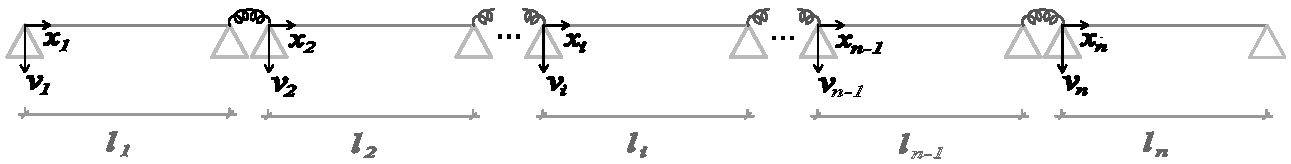
\includegraphics[width=1\textwidth]{Figures/model1.pdf}
    \caption{Beam-spring system.}
    \label{fig:sketch}
\end{figure}


\noindent Applying \textit{Newton's second law of motion} to the infinitesimal element of a beam and considering the coordinate system centered in the initial section of the beam, the equation of motion  is:

\begin{equation}
    \rho A \dfrac{\partial^2 v(x,t)}{\partial t^2} + EI\dfrac{\partial^4 v(x,t)}{\partial x^4}=0
    \label{eq1}
\end{equation}

\noindent where $v(x,t)$ is the vertical displacement of the beam. It is searched a solution of Eq.\ref{eq1} in the form:
\begin{equation}
    v(x,t)= u(x) sin(\omega t)
    \label{solv}
\end{equation}

\noindent The derivatives of $v(x,t)$ are:
\begin{subequations}
\begin{equation}
    \dfrac{\partial^2 v}{\partial t^2} = -\omega^2 u(x) \sin \ \omega t  %\dfrac{\partial^2 v}{\partial t^2} = -\omega^2 u(x) sin \ \omega t \\
    \label{eq3}
\end{equation} 
\begin{equation}
    \dfrac{\partial^4 v}{\partial x^4} = \dfrac{d^4 u}{d x^4} sin \ \omega t
\label{eq4}
\end{equation} 
\end{subequations}
By substituting Eqs.\ref{eq3} and \ref{eq4}, Eq.\ref{eq1} becomes:

\begin{equation}
     \dfrac{d^4 u(x)}{d x^4} \ -  \ \omega^2  \ \dfrac{\rho A}{EI} \ u(x) \ = \ 0
\end{equation}

\noindent that can be solved in the form:
\begin{equation}
\dfrac{d^4 u(x)}{d x^4} - \alpha^4 u(x) = 0 \; \; \; where \; \; \; \alpha = ^4\sqrt{\omega^2 \dfrac{\rho A}{EI}} 
\label{eq6}
\end{equation}

\noindent The solution of Eq.\ref{eq6} is:

\begin{equation}
u(x) = C \ cos\ \alpha x   + D \ sin\ \alpha x   + E \ cosh\ \alpha x   + F \ sinh\ \alpha x  
\label{sol}
\end{equation}
To solve the system of equation it is necessary to write the boundary conditions; since the constraints don't vary with respect to time it is possible to apply the boundary conditions directly in equation (\ref{sol}).\newline
Considering a system composed by $n$ simply supported beams which are characterized by the same geometrical and mechanical characteristics, it is necessary to write $n$ equations of motion in the form given by Eq. \ref{eq1}), then it is generated an \textit{homogeneous n-dimensional partial differential system of equation}:

\begin{equation}
     \begin{cases}
    \rho A \dfrac{\partial^2 v_1(x_1,t)}{\partial t^2} + EI\dfrac{\partial^4 v_1(x_1,t)}{\partial x_1^4}=0\\
    \rho A \dfrac{\partial^2 v_2(x_2,t)}{\partial t^2} + EI\dfrac{\partial^4 v_2(x_2,t)}{\partial x_2^4}=0\\
    \hspace{2cm} \vdots\\
    \rho A \dfrac{\partial^2 v_i(x_i,t)}{\partial t^2} + EI\dfrac{\partial^4 v_i(x_i,t)}{\partial x_i^4}=0\\
    \hspace{2cm} \vdots\\
    \rho A \dfrac{\partial^2 v_n(x_n,t)}{\partial t^2} + EI\dfrac{\partial^4 v_n(x_n,t)}{\partial x_n^4}=0
    \end{cases}
    \label{eq:diff1}
\end{equation}

\noindent The solution of Eq. \ref{eq:diff1} is:
\begin{equation}
    \begin{cases}
    u_1(x_1) = C_1 \ cos\ \alpha x_1   +  D_1 \ sin\ \alpha x_1   + E_1 \ cosh\ \alpha x_1   + F_1 \ sinh\ \alpha x_1\\
    u_2(x_2) = C_2 \ cos\ \alpha x_2   +  D_2 \ sin\ \alpha x_2   + E_2 \ cosh\ \alpha x_2   + F_2 \ sinh\ \alpha x_2\\
    \hspace{4.5cm} \vdots\\
    u_i(x_i) \ = C_i \ cos\ \alpha x_i  \  +  D_i \ sin\ \alpha x_i   \  + E_i \ cosh\ \alpha x_i  \  + F_i \ sinh\ \alpha x_i\\
    \hspace{4.5cm} \vdots\\
    u_n(x_n) = C_n \ cos\ \alpha x_n   +  D_n \ sin\ \alpha x_n   + E_n \ cosh\ \alpha x_n   + F_n \ sinh\ \alpha x_n
    \end{cases}
    \label{eq7}
\end{equation}

\noindent According with the assumptions defined previously, the \textit{boundary conditions} are the following:
\begin{subequations}
\begin{equation}
u_i(0) \  = \ 0
\label{BC1}
\end{equation}
\begin{equation}
u_i(l_i) \ = \ 0
\label{BC2}
\end{equation}
\begin{equation}
u_i''(l_i)\ =\  u_{i+1}''(0)
\label{BC3}
\end{equation}
\begin{equation}
u_i''(l_i) \ = \ \beta  \ \big( \ u'_{i+1}(0)\ -\ u'_{i}(l_i) \ \big)
\label{BC4}
\end{equation}
\label{BCS}
\end{subequations}
where $\beta = \dfrac{K}{EI}$ is the \textit{connection degree} of the system.\\

\noindent The result of Eq.\ref{BC1} is $E_i = - C_i$. Then Eq.\ref{eq7} can be wrote as: 

\begin{equation}
    u_i(x) = C_i \ ( cos \ \alpha x - cosh\ \alpha x   ) + D_i \ sin\ \alpha x   + F_i \ sinh\ \alpha x
    \label{equi}
\end{equation}
and the derivatives are:
\begin{equation}
     u_i'(x) = \alpha \ (- C_i (sin\ \alpha x  + sinh\ \alpha x   ) + D_i \ cos\ \alpha x   + F_i \ cosh\ \alpha x  )
    \label{der1}
\end{equation}
\begin{equation}
    u_i''(x) = \alpha^2 \ (- C_i \ ( cos\ \alpha x   + cosh\ \alpha x   ) - D_i \  sin\ \alpha x   + F_i \ sinh\ \alpha x  )
    \label{der1}
\end{equation}

\noindent Eqs.\ref{BC2}, \ref{BC3} and \ref{BC4} becomes respectively:
\begin{subequations}
    \begin{align}
 C_i \ \big( cos\ \alpha l_i - cosh\ \alpha l_i\  \big) \ + D_i \ sin\ \alpha l_i\  + F_i \ sinh\ \alpha l_i\  \ & = &\ 0\\
C_i \ ( cos\ \alpha l_i\ + cosh\ \alpha l_i\ )   + D_i sin\ \alpha l_i\  - F_i \ sinh\ \alpha l_i\ ) & = & 2 \ C_{i+1}\\
\beta \ \big ( D_{i+1} + F_{i+1} +  C_i \ (sin\ \alpha l_i\  - sinh\ \alpha l_i\  ) - D_i\  cos\ \alpha l_i\  - F_i \ cosh\ \alpha l_i\  \big) & = & - \ 2 \  \alpha \ C_{i+1}
    \end{align}
    \label{eq12}
\end{subequations}
\noindent Adding Eq.\ref{eq12}a to Eq.\ref{eq12}b: 
\begin{equation}
    2 \ C_i \ cos \ \alpha l_i \ + \ 2 \ D_i \ sin \ \alpha l_i  = 2 \ C_{i+1} \, \, \xrightarrow{} D_i \ = \ \dfrac{C_{i+1} \ - \ C_i \ cos\ \alpha l_i}{sin\ \alpha l_i}
    \label{eqD}
\end{equation}
\noindent Subtracting Eq.\ref{eq12}b from Eq.\ref{eq12}a:
\begin{equation}
    - 2 \ C_i \ cosh \ \alpha l_i \  + \ 2 \ F_i \ sinh \ \alpha l_i\  = -2 \ C_{i+1} \, \, \xrightarrow{} F_i = \dfrac{-C_{i+1} + C_i \ cosh \ \alpha l_i}{sinh\ \alpha l_i}
    \label{eqF}
\end{equation}


\noindent By substituting Eq.\ref{eqD} and Eq.\ref{eqF} in Eq.\ref{eq12}c:

\begin{equation}
    D_{i+1} \ + \ F_{i+1} \ - \ C_i \ ( \ cosech\ \alpha l_i\ -  \ cosec\ \alpha l_i\ ) \ + \ C_{i+1} \ ( \ cotanh\ \alpha l_i\ - \ cotan\ \alpha l_i \ ) \ = \ - \ 2 \  \dfrac{\alpha}{\beta} \ C_{i+1}
     \label{eq15}
\end{equation}
Establishing the following parameters:
\begin{subequations}
\begin{equation}
 \phi_i \ = \  cotanh \ \alpha l_i\  - \ cotan\ \alpha l_i
\end{equation}
\begin{equation}
 \psi_i \ = \ cosech\ \alpha l_i\  - \ cosec\ \alpha l_i
\end{equation}
\end{subequations}
Eq.\ref{eq15} becomes:
\begin{equation}
    D_{i+1} \ + \ F_{i+1} \ - \ C_i \ \psi_i \ + \ C_{i+1} \ \phi_i \ = \ - \ 2 \  \dfrac{\alpha}{\beta} \ C_{i+1}
    \label{eq16}
\end{equation}
It is easily demonstrable that the sum of $D_i$ and $F_i$ is:
\begin{equation}
D_i \ + \ F_i \ = \ C_i \ \phi_i - C_{i+1} \ \psi_i 
\label{eqsum}
\end{equation}
By substituting Eq.\ref{eqsum} in Eq.\ref{eq16} it is possible to find the solution:
\begin{equation}
    C_i \ (\ - \psi_i \ ) \ + \ C_{i+1}\ ( \ \phi_i \ + \ \phi_{i+1} \ + \ 2 \  \dfrac{\alpha}{\beta} \ ) \  - \ C_{i+2} \ \psi_{i+1} \ = \ 0
    \label{eqsol}
\end{equation}

\noindent It is necessary to adopt an extremity boundary condition to define the annulment of curvature in the initial and ending sections of the first and last spans, respectively.
In particular, it is necessary to impose the conditions that follow:
\begin{equation}
    \begin{cases}
    \dfrac{d^2 \ u_1(0)}{dx_1^2} \ = \ 0\\
    \\
    
    \dfrac{d^2 \ u_n(l_n)}{dx_n^2} \ = \ 0\\
    \end{cases}
    \, \ ,\xrightarrow{} \, \, 
    \begin{cases}
     C_1 \ = \ 0\\
     \\
     C_{n+1} \ = \ 0 
    \end{cases}
\end{equation}

\noindent Hence, Eqs.\ref{eqsol} is a system composed by (n-1) equations (an equation for each internal support) that can be expressed in the form:
\begin{equation}
    \begin{bmatrix}
     \  \phi_1\  + \ \phi_2 \ + \ 2 \ \dfrac{\alpha}{\beta} & -\psi_2 &  0  & \cdots &  0  & 0 \\
       -\psi_2  &   \phi_2\  + \ \phi_3 \ + \ 2 \ \dfrac{\alpha}{\beta}  &  -\psi_3    &  \cdots  & 0  & 0\\
        0   &   -\psi_3  &   \phi_3\  + \ \phi_4 \ + \ 2 \ \dfrac{\alpha}{\beta}   & \cdots &  0 &  0\\
        \vdots  & \vdots   & \vdots  &  & \vdots & \vdots \\
        0  & 0  & 0   & \cdots &  -\psi_{n-1}  &   \phi_{n-1}\  + \ \phi_n \ + \ 2 \ \dfrac{\alpha}{\beta} \; 
    \end{bmatrix}
    \begin{Bmatrix}
      C_2 \\
      \\
      C_3 \\
      \\
      C_4 \\
      \\
      \vdots \\
      \\
      C_{n}
    \end{Bmatrix}
    \ = \ 
    \begin{Bmatrix}
    0 \\
      \\
      0 \\
      \\
      0 \\
      \\
      \vdots \\
      \\
      0
    \end{Bmatrix}
    \label{eq20}
\end{equation}
\noindent A condensed form of Eq.\ref{eq20} is:
\begin{equation}
    \textbf{M C} \ = \ \textbf{0}
    \label{eq:linsys}
\end{equation}
\noindent If it is imposed that: $l_i = l_{i+1} = ... = l_n =  L$ and $\Lambda =\alpha L$ then Eqs.\ref{eqsol} become:
\begin{equation}
    -C_i\  \psi + 2 \ C_{i+1} \ ( \phi +\dfrac{\Lambda}{\beta L}) \ - \ C_{i+2} \psi \ = \ 0
\end{equation}
and the matrix of coefficients $\textbf{M}$ is:
\begin{equation}
    \begin{bmatrix}
      2 \ \bigg( \ \phi \ + \ \dfrac{\Lambda}{\beta L} \ \bigg) & -\psi &  0  & 0 & \cdots &  0  & 0 \\
       -\psi  &   2 \ \bigg( \ \phi \ + \ \dfrac{\Lambda}{\beta L} \ \bigg)  &  -\psi  &   0  &  \cdots  & 0  & 0\\
        0   &   -\psi  &   2 \ \bigg( \ \phi \ +\ \dfrac{\Lambda}{\beta L} \ \bigg)  &  -\psi  & \cdots &  0 &  0\\
       \vdots  & \vdots  & \vdots  & \vdots  &  & \vdots & \vdots\\
        0  & 0  & 0  & 0  & \cdots &  -\psi  & 2 \ \bigg( \ \phi \ +\ \dfrac{\Lambda}{\beta L} \ \bigg)
    \end{bmatrix}
\end{equation}
\noindent Since $\alpha$ has dimensions $[L^{-1}]$, $\Lambda$ is a non-dimensional value. Eq. \ref{eq:linsys} is an \textit{homogeneous linear system of equations}. 
The eigenvalues solution is determined by the annulment of the determinant of the $(n-1)\cdot(n-1)$ matrix of coefficients $\textbf{M}$, that permits to find $\Lambda$ values and then $\alpha$. By substituting $\Lambda$ in Eq.\ref{eq6} it is possible to find the eigenvalues $\omega$ and the natural frequencies $f$ of the system as:
\begin{equation}
    \omega \ = \  \sqrt{\dfrac{\Lambda^4}{L^4}\dfrac{E I}{\rho A}} \ \; \; \; \; \;
          f\ = \ \sqrt{\dfrac{\Lambda^4}{4 \ \pi^2 \ L^4}\dfrac{E I}{\rho A}}
    \label{eq:eigen}
\end{equation}

\noindent Looking at Eq.\ref{eqsol} it is clear that the effect on the final solution given by the rotational springs is totally expressed by  $\beta L$ which is a non-dimensional value that represent the ratio between the stiffness of the springs $K$ and the stiffness of the beam $EI/L$.\newline 
If the stiffness of the beam $EI/L$ is much greater than $K$, then $\beta L \xrightarrow{}\infty$, solution converges to the continuous multi-span simply supported beam solution. On the other hand, if $\beta L \xrightarrow{}0$ then Eq.\ref{eqsol} lose its signification and tends to an indeterminate equation. In fact if the connection between the spans is null, then Eq.\ref{BC4} becomes a boundary condition that expliques a null value of bending moment over the internal supports. In particular, it is possible to demonstrate that solutions of the single simply supported beam problem are:
\begin{equation}
    \Lambda = h \pi  \ \ \ C_i=0   \ \ \  E_i=0   \ \ \ F_i=0   \ \ \ D_i = \left(\dfrac{2}{L}\right)^{1/2}
\end{equation}

\noindent Determinant of the matrix of coefficients $\textbf{M}$ is a transcendent function, then solutions must be found numerically.\newline
In Figure \ref{fig:2345spans} it is possible to see the graph of $det(\textbf{M})$ - $\Lambda$ for various $n$ cases and $\beta L$ equal to 5. Intersections between $det(\textbf{M})$ functions and the abscissa axis are solutions in terms of $\Lambda$. By comparing Figure \ref{fig:2345spans} and Tab. \ref{tab:res2345} it is clear that recursive asymptotic solutions proportional to $\pi$ occur (dashed red lines in Figure \ref{fig:2345spans}).Therefore, groups of solutions that are in a small distance from $\Lambda = h \pi$  can be defined, and each one is composed by $n$ solutions. If $\beta L$ increases the gap between the solutions increases too, until reaching the maximum gap for $\beta L\xrightarrow{}\infty$. On the other hand, if $\beta L\xrightarrow{}0$ each beam becomes an independent simply supported beam and all eigenvalues converge to the same values.

\begin{figure}[H]
    \centering
    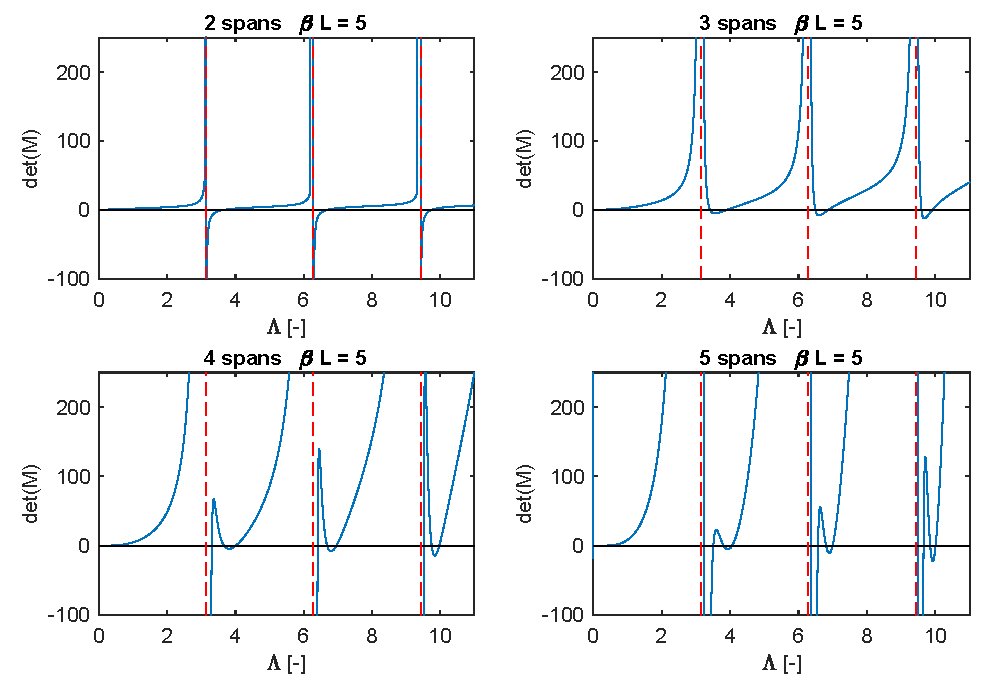
\includegraphics[width=0.9\textwidth]{Figures/graphs2345.pdf}
    \caption{Graphs of $det(\textbf{M})=0$ in the case of 2, 3, 4 and 5 spans and $\beta L=5$.}
    \label{fig:2345spans}
\end{figure}
\begin{table}[H]
    \centering
    \begin{tabular}{c c c c }
         2 spans & 3 spans & 4 spans & 5 spans \\
         \midrule
         3.1416 & 3.1416 & 3.1416 & 3.1416 \\
         3.6646 & 3.4145 & 3.3052 & 3.2497 \\
                & 3.9071 & 3.6646 & 3.5118 \\
                &        & 4.0084 & 3.8146 \\
                &        &        & 4.0590 \\
         6.2832 & 6.2832 & 6.2832 & 6.2832 \\
         6.6874 & 6.4929 & 6.4086 & 6.3659 \\
                & 6.8767 & 6.6874 & 6.5683 \\
                &        & 6.9553 & 6.8045 \\
                &        &        & 6.9943 \\
         9.4248 & 9.4248 & 9.4248 & 9.4248 \\
         9.7516 & 9.5921 & 9.5241 & 9.4900 \\
                & 9.9081 & 9.7516 & 9.6536 \\
                &        & 9.9730 & 9.8484 \\
                &        &        & 10.0051 \\
    \end{tabular}
    \caption{Solutions of $det(\textbf{M})=0$ in the domain of [0 11] for $\beta L = 5$ in the case of 2, 3, 4 and 5 spans.}
    \label{tab:res2345}
\end{table}

}
\begin{figure}[H]
    \centering
    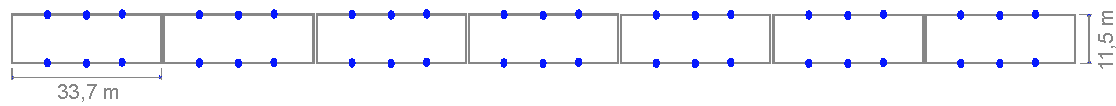
\includegraphics[width=1\textwidth]{Figures/bridge_sketch_downey.pdf}
    \caption{Bridge sketch. Blue points define the position of the accelerometers.}
\end{figure}
\begin{figure}[H]
    \centering
    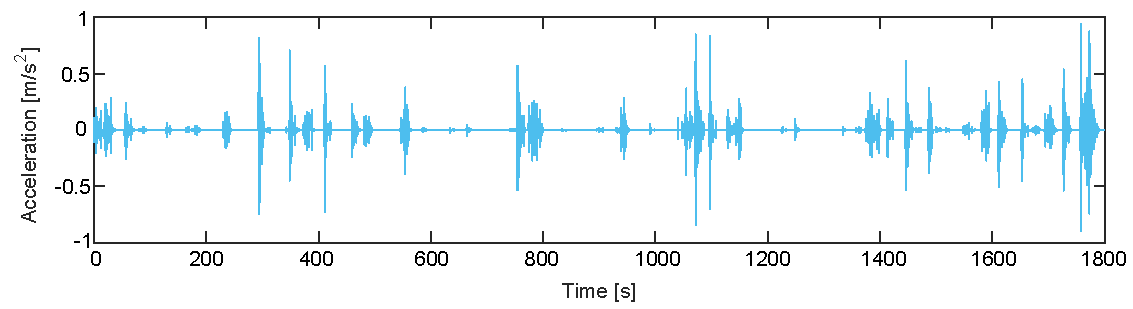
\includegraphics[width=1\textwidth]{Figures/timehistories_downey.pdf}
    \caption{Example of time history.}
\end{figure}
\begin{figure}[H]
    \centering
    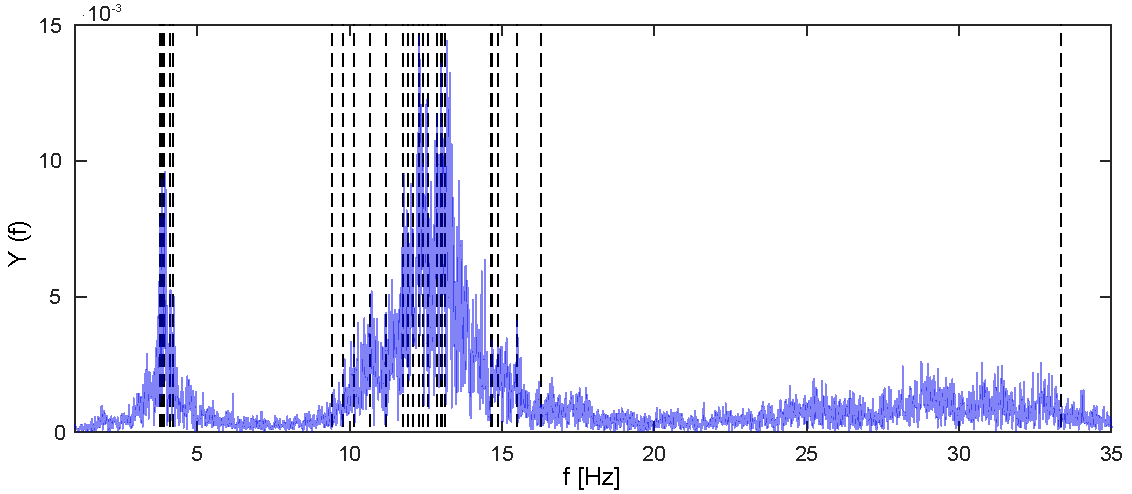
\includegraphics[width=1\textwidth]{Figures/fft_downey.pdf}
    \caption{Fast Fourier Transform Y(f) of the signal. Dashed lines are the identified frequencies through OMA.}
\end{figure}

\end{document}
